\chapter{Framing and Codecs: Putting Message Boundaries Back}\label{ch:framing}

\begin{objectives}
\begin{itemize}
\item compare delimiter, length-prefix and self-describing framing;
\item encode a concrete VaR request byte by byte: payload, big-endian prefix, full hex dump;
\item specify the decoder as a state machine and \emph{prove} it reconstructs frames under every segmentation;
\item defend a server against hostile length prefixes;
\item explain what a binary codec changes (fixed-width fields, byte order, varints) and why only the codec changes.
\end{itemize}
{\small\color{muted}\textbf{Chapter references:} Protocol Buffers encoding guide~\cite{protobuf}; nlohmann/json~\cite{nlohmannjson};
Stevens et al.~\cite{stevens2004unp}.}
\end{objectives}

\section{Three ways to mark a boundary}
\Cref{prop:boundary} says TCP will not tell us where messages end, so the bytes must. There are three classic answers.

\begin{center}
\small
\begin{tabularx}{\linewidth}{@{}>{\leavevmode\bfseries\color{yel}}p{2.6cm} X X@{}}
\toprule
\textcolor{muted}{Strategy} & \textcolor{muted}{Mechanism} & \textcolor{muted}{Cost / risk}\\
\midrule
Delimiter & A reserved byte sequence ends each message (newline-delimited JSON; CRLF after HTTP/1.1 header lines). & Payload must escape the delimiter; the decoder scans every byte.\\
Length prefix & A fixed-size header carries the payload length. & Decoder jumps straight to the end; the length is attacker-controlled (\cref{sec:maxframe}).\\
Self-describing & Every field is tagged with its type and length (TLV; Protocol Buffers~\cite{protobuf}). & Most flexible, most complex; still needs an outer frame on a stream.\\
\bottomrule
\end{tabularx}
\end{center}

Decision D5 chose a length prefix: four bytes, unsigned, big-endian, followed by JSON.

\repo[firstline=9,lastline=31]{include/score/net/codec.hpp}{The codec interface. \cc{encode} is pure; \cc{feed} and
\cc{try_decode} split decoding into ``accept bytes'' and ``extract a frame if one is complete'', which is exactly the
shape \cref{thm:segmentation} needs.}{lst:codec}

\repo[firstline=9,lastline=21]{include/score/net/json_codec.hpp}{The v1 codec. Its only state is \cc{buffer_}: the
bytes received but not yet consumed.}{lst:jsoncodec}

\section{Encoding a request, byte by byte}\label{sec:encode}
\begin{definition}[Big-endian unsigned 32-bit integer]
Bytes $b_0b_1b_2b_3$ encode $N=b_0\cdot 2^{24}+b_1\cdot 2^{16}+b_2\cdot 2^{8}+b_3$. Most significant byte first is also
called \emph{network byte order}.
\end{definition}

Take the pre-trade request ``95\% VaR for AAPL'', built as
\begin{center}\cc{nlohmann::json{{"op","var"},{"symbol","AAPL"},{"conf",0.95}}}.\end{center}
We ran it through a reference encoder built
on the repository's own \texttt{nlohmann/json}~3.12.0 submodule (\file{verify/codec_test.cpp}).

\begin{progout}{codec\_test: encoding the request}{lst:encodeout}
dump: {"conf":0.95,"op":"var","symbol":"AAPL"}
len=40 total=44
hex:
  00 00 00 28 7B 22 63 6F 6E 66 22 3A 30 2E 39 35
  2C 22 6F 70 22 3A 22 76 61 72 22 2C 22 73 79 6D
  62 6F 6C 22 3A 22 41 41 50 4C 22 7D
\end{progout}

Three details deserve attention.
\begin{enumerate}[label=\textbf{\color{yel}\arabic*.}]
\item \textbf{Key order changed.} \cc{nlohmann::json}'s default object type is \cc{std::map<std::string, json>},
so \cc{dump()} emits keys \emph{sorted}: \texttt{conf}, \texttt{op}, \texttt{symbol}. Any test that
compares encoded bytes against a hand-written string must account for this.
\item \textbf{Compact output.} \cc{dump()} with no indent emits no spaces or newlines: 40 bytes, so $N=40=\hex{0x28}$
and the prefix is \hex{00 00 00 28}.
\item \textbf{The number is text.} \texttt{0.95} travels as the four ASCII bytes \hex{30 2E 39 35}. The receiver parses
them back to the binary64 value nearest $0.95$, which is $0.9499999999999999555\ldots$ (\cref{ch:float}).
\end{enumerate}

\begin{figure}[htbp]
\centering
\begin{tikzpicture}[x=0.92cm,y=0.95cm]
\def\row#1#2{\foreach \b [count=\i from 0] in {#2}{\node[byte] at (\i,-#1) {\b};}}
\foreach \i/\b in {0/00,1/00,2/00,3/28}{\node[byte,draw=yel,text=yel,fill=yel!12!bg] at (\i,0) {\b};}
\foreach \b [count=\i from 4] in {7B,22,63,6F,6E,66,22,3A,30,2E,39,35}{\node[byte,draw=acc] at (\i,0) {\b};}
\foreach \b [count=\i from 0] in {2C,22,6F,70,22,3A,22,76,61,72,22,2C,22,73,79,6D}{\node[byte,draw=acc] at (\i,-1) {\b};}
\foreach \b [count=\i from 0] in {62,6F,6C,22,3A,22,41,41,50,4C,22,7D}{\node[byte,draw=acc] at (\i,-2) {\b};}
% ascii under
\foreach \c [count=\i from 4] in {\{,",c,o,n,f,",:,0,.,9,5}{\node[font=\scriptsize\ttfamily,text=muted] at (\i,0.55) {\c};}
\foreach \c [count=\i from 0] in {{,},",o,p,",:,",v,a,r,",{,},",s,y,m}{\node[font=\scriptsize\ttfamily,text=muted] at (\i,-0.45) {\c};}
\foreach \c [count=\i from 0] in {b,o,l,",:,",A,A,P,L,",\}}{\node[font=\scriptsize\ttfamily,text=muted] at (\i,-1.45) {\c};}
\foreach \o [count=\r from 0] in {0,16,32}{\node[font=\scriptsize\ttfamily,text=codeframe!50!muted,anchor=east] at (-0.6,-\r) {+\o};}
\draw[decorate,decoration={brace,amplitude=5pt,mirror},draw=yel] (-0.45,-2.5) -- (3.45,-2.5) node[midway,below=6pt,font=\footnotesize,text=yel,align=center]{length prefix\\ $0\cdot2^{24}+0\cdot2^{16}+0\cdot2^{8}+40$};
\draw[decorate,decoration={brace,amplitude=5pt,mirror},draw=acc] (3.55,-2.5) -- (11.45,-2.5) node[midway,below=6pt,font=\footnotesize,text=acc,align=center]{payload: 40 bytes\\ (12 in row +0, 16 in row +16, 12 in row +32)};
\end{tikzpicture}
\caption{The 44-byte frame, 16 bytes per row (TikZ). Yellow: length prefix. Blue: UTF-8 JSON payload, with the ASCII
character above each byte.}
\label{fig:frame}
\end{figure}

\section{The decoder as a state machine}
\begin{figure}[htbp]
\centering
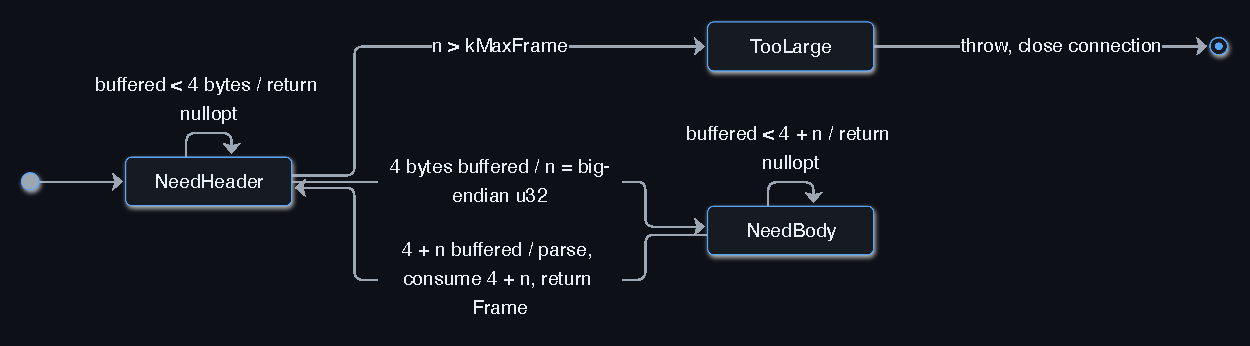
\includegraphics[width=0.92\linewidth]{diagrams/decoder_state.pdf}
\caption{Decoder states (Mermaid). Note that the decoder never needs a separate ``in the middle of a frame'' flag: the
state is a function of the buffered bytes alone.}
\label{fig:decoderstate}
\end{figure}

\Cref{lst:sketch} is a reference implementation, written for this tutorial and \emph{not} part of the repository, whose
\cc{JsonFrameCodec} still throws (\cref{lst:jsonstub}). It differs from the repository's header only in carrying a read
offset \cc{pos_} so that consuming a frame does not shift the buffer (\cref{ex:quadratic}).

\begin{code}{codec\_sketch.hpp: a reference length-prefixed JSON codec}{lst:sketch}
class SketchJsonFrameCodec {
public:
    static constexpr std::uint32_t kMaxFrame = 1u << 20;  // 1 MiB

    std::vector<std::uint8_t> encode(const Frame& f) const {
        const std::string body = f.payload.dump();
        const auto n = static_cast<std::uint32_t>(body.size());
        std::vector<std::uint8_t> out{
            static_cast<std::uint8_t>(n >> 24), static_cast<std::uint8_t>(n >> 16),
            static_cast<std::uint8_t>(n >> 8),  static_cast<std::uint8_t>(n)};
        out.insert(out.end(), body.begin(), body.end());
        return out;
    }

    void feed(const std::uint8_t* data, std::size_t len) {
        buf_.insert(buf_.end(), data, data + len);
    }

    std::optional<Frame> try_decode() {
        if (buf_.size() - pos_ < 4) return std::nullopt;            // HEADER: need 4 bytes
        const std::uint8_t* p = buf_.data() + pos_;
        const std::uint32_t n = (std::uint32_t{p[0]} << 24) | (std::uint32_t{p[1]} << 16) |
                                (std::uint32_t{p[2]} << 8)  |  std::uint32_t{p[3]};
        if (n > kMaxFrame) throw std::length_error("frame too large");
        if (buf_.size() - pos_ - 4 < n) return std::nullopt;        // BODY: need n bytes
        Frame f{nlohmann::json::parse(p + 4, p + 4 + n)};
        pos_ += 4 + n;
        if (pos_ == buf_.size()) { buf_.clear(); pos_ = 0; }        // compact when drained
        return f;
    }

private:
    std::vector<std::uint8_t> buf_;
    std::size_t pos_ = 0;
};
\end{code}

\section{Correctness under arbitrary segmentation}
\begin{theorem}[Segmentation invariance]\label{thm:segmentation}
Let $f_1,\dots,f_m$ be frames whose encodings $e_j=\mathrm{enc}(f_j)$ satisfy $|e_j|-4\le$ \cc{kMaxFrame}, and let
$S=e_1\Vert\cdots\Vert e_m$. Partition $S$ into consecutive chunks $c_1,\dots,c_q$ (any $q\ge1$, any lengths, empty chunks
allowed). Run, for $i=1,\dots,q$: \cc{feed}$(c_i)$, then call \cc{try_decode} until it returns \cc{nullopt}. Then the
frames returned, in order, are exactly $f_1,\dots,f_m$, and afterwards the buffer is empty.
\end{theorem}

\begin{proof}
Let $E_j=|e_1|+\cdots+|e_j|$ (so $E_0=0$), let $F$ be the number of bytes fed so far, and let $d$ be the number of frames
returned so far. We claim the following invariant holds between calls:

\smallskip
\textbf{(I)} the unconsumed bytes \cc{buf_[pos_..)} equal $S[E_d, F)$, and the frames returned are $f_1,\dots,f_d$.

\smallskip
\emph{Initially} $d=F=0$ and the buffer is empty, so (I) holds. \emph{\cc{feed}} appends $c_i$, which is $S[F,F+|c_i|)$
because chunks are consecutive, and leaves $d$ unchanged; (I) holds with the new $F$. \emph{\cc{try_decode}}: let
$U=S[E_d,F)$ be the unconsumed bytes. If $|U|<4$ it returns \cc{nullopt} and changes nothing. Otherwise, by (I), the
first four bytes of $U$ are the first four bytes of $e_{d+1}$, that is, the prefix of $f_{d+1}$, so the decoded $n$ is
$|e_{d+1}|-4\le$ \cc{kMaxFrame} and no exception is thrown. If $|U|<4+n$ it returns \cc{nullopt}. Otherwise
$U[4,4+n)$ is exactly the payload of $f_{d+1}$, so it returns $f_{d+1}$ and advances \cc{pos_} by $4+n=|e_{d+1}|$;
the unconsumed bytes become $S[E_{d+1},F)$ and (I) holds with $d+1$. The compaction branch only discards
already-consumed bytes and preserves (I).

\emph{Termination}: each successful call consumes at least 4 bytes, so each inner loop ends. \emph{Completeness}: after
the last chunk, $F=|S|=E_m$. If $d<m$ then $U=S[E_d,E_m)$ begins with the whole of $e_{d+1}$, so the next call succeeds.
The loop therefore stops only when $d=m$, at which point $U$ is empty.
\end{proof}

\begin{remarkbox}
The proof uses one property of the decoder: its decision depends only on the bytes buffered so far, and more bytes
never turn a ``complete'' answer into ``incomplete''. Any framing with that \emph{prefix-monotone} property, such as
newline delimiting with escaped payloads, admits the same proof.
\end{remarkbox}

\begin{verified}
\file{verify/codec_test.cpp} concatenates the request with a second frame,
\texttt{\{"conf":0.975,"op":"cvar","symbol":"MSFT"\}} (42-byte payload), into a 90-byte stream and checks
\emph{every} split into three consecutive chunks, i.e.\ every pair $0\le i\le j\le 90$:
$\binom{92}{2}=4186$ cases, all decoding to the two original frames. Feeding one byte at a time also yields exactly two
frames.
\end{verified}

\begin{example}[One frame across three reads]\label[example]{ex:threereads}
Suppose the 44 bytes of \cref{fig:frame} arrive as reads of 3, 20 and 21 bytes, as they did on loopback in
\cref{lst:streamout}. The decoder's view:
\begin{center}
\small
\begin{tabular}{@{}clrll@{}}
\toprule
\textcolor{muted}{read} & \textcolor{muted}{bytes received} & \textcolor{muted}{buffered} & \textcolor{muted}{state} & \textcolor{muted}{\cc{try_decode}}\\
\midrule
1 & \hex{00 00 00} & 3 & need header ($3<4$) & \cc{nullopt}\\
2 & \hex{28 7B 22 \dots\ 22 3A 22} & 23 & header read, $n=40$; need $44$ & \cc{nullopt}\\
3 & \hex{76 61 72 \dots\ 4C 22 7D} & 44 & complete & frame; buffer cleared\\
\bottomrule
\end{tabular}
\end{center}
Notice that the length prefix itself was split: read 1 delivered three of its four bytes. A decoder that read the length
from ``the first four bytes of this read'' would have computed $\hex{0x00000028}$ only by luck in some runs and garbage in
others. The run of \file{verify/codec_test.cpp} printed \texttt{nullopt}, \texttt{nullopt}, and the decoded object for the
three reads, in agreement with the table.
\end{example}

\begin{figure}[htbp]
\centering
\begin{tikzpicture}[x=0.3cm,y=0.9cm]
\foreach \i in {0,...,3}{\draw[draw=yel,fill=codebg] (\i,0) rectangle ++(1,0.7);}
\foreach \i in {4,...,43}{\draw[draw=acc,fill=codebg] (\i,0) rectangle ++(1,0.7);}
\fill[yel!35!codebg] (0.05,0.05) rectangle (3.95,0.65);
\draw[very thick,red] (3,-0.25) -- (3,0.95);
\draw[very thick,red] (23,-0.25) -- (23,0.95);
\node[font=\footnotesize,text=fg] at (1.5,1.35) {read 1};
\node[font=\footnotesize,text=fg] at (13,1.35) {read 2: 20 bytes};
\node[font=\footnotesize,text=fg] at (33.5,1.35) {read 3: 21 bytes};
\node[font=\scriptsize,text=yel,anchor=north] at (2,-0.3) {prefix};
\node[font=\scriptsize,text=red,anchor=north] at (13,-0.3) {cuts at byte 3 and byte 23};
\node[font=\scriptsize,text=muted,anchor=north] at (36,-0.3) {payload ends at byte 44};
\end{tikzpicture}
\caption{The split of \cref{ex:threereads} (TikZ). The first cut falls inside the length prefix.}
\label{fig:threereads}
\end{figure}

\section{Defending against hostile lengths}\label{sec:maxframe}
The length prefix is chosen by whoever is on the other end of the socket. Without a bound, the four bytes
\hex{FF FF FF FF} announce a $4{,}294{,}967{,}295$-byte payload, almost exactly 4\,GiB.

\begin{pitfall}[title={Pitfall: trusting the prefix}]
A decoder that does \cc{buffer.reserve(n)} as soon as it reads $n$ lets one 4-byte message from any client allocate
4\,GiB. A decoder that merely waits for $n$ bytes lets a client grow the buffer without limit by sending slowly. Both are
denial-of-service bugs.
\end{pitfall}

\begin{proposition}[Per-connection memory bound]\label[proposition]{prop:membound}
With the check \cc{n > kMaxFrame} in place, and reads of at most $R$ bytes fed only while \cc{try_decode} has been
drained, a connection's buffered bytes never exceed $4+\text{\cc{kMaxFrame}}+R$.
\end{proposition}
\begin{proof}
After draining, the unconsumed bytes are a proper prefix of one frame (else another frame would decode), so they number at
most $4+n-1\le 3+\text{\cc{kMaxFrame}}$, or the header check has thrown. One more read adds at most $R$.
\end{proof}

The bound covers memory, not time: a client can hold a partial frame open forever and tie up a descriptor. That needs an
idle timeout, which belongs to \cc{Connection}, not to the codec. The verification program also checked that the prefix
\hex{7F FF FF FF} ($2{,}147{,}483{,}647$) makes \cc{try_decode} throw \cc{std::length_error} before any allocation.

\section{Toward a binary codec}
JSON spends bytes on punctuation and field names and turns every number into decimal text. A binary codec (Phase 8)
replaces this with fixed-width fields and explicit byte order, and optionally \emph{varints}.

\begin{definition}[Base-128 varint]\label[definition]{def:varint}
An unsigned integer is written in 7-bit groups, least significant group first; every byte except the last has its high
bit set. Protocol Buffers uses this encoding, mapping signed integers through the zig-zag transform
$z(v)=2v$ for $v\ge0$ and $z(v)=-2v-1$ for $v<0$ so that small negative numbers stay short~\cite{protobuf}.
\end{definition}

\begin{verified}
Encodings computed by \file{verify/encodings.py}: $40\mapsto$ \hex{28}; $127\mapsto$ \hex{7F};
$128\mapsto$ \hex{80 01}; $300\mapsto$ \hex{AC 02}; $9500\mapsto$ \hex{9C 4A}. Zig-zag: $-1\mapsto1$, $1\mapsto2$.
As a fixed-width big-endian \texttt{u16}, $9500$ is \hex{25 1C} and $9750$ is \hex{26 16}.
\end{verified}

A binary layout for the same request could be: one byte of opcode, one byte of symbol length, the symbol's ASCII bytes,
and the confidence as a \texttt{u16} in basis points:
\hex{01}\,\textbar\,\hex{04}\,\textbar\,\hex{41 41 50 4C}\,\textbar\,\hex{25 1C}: 8 payload bytes instead of 40, and, as
\cref{ch:float} will show, a confidence that is an exact integer instead of an inexact binary fraction.

\repo[firstline=13,lastline=22]{include/score/net/server.hpp}{\cc{CodecFactory} is why only the codec changes: \cc{Server}
asks the factory for one codec per connection and never names a concrete codec type. Switching to binary means passing a
different lambda at the call site that constructs \cc{Server}.}{lst:codecfactory}

\begin{exercises}
\ex{ex:cvarframe}{\lvA} Encode \texttt{\{"op":"cvar","symbol":"MSFT","conf":0.975\}} by hand, remembering that
\cc{dump()} sorts keys. Give the payload length, the four prefix bytes, and the first eight payload bytes in hex.

\ex{ex:quadratic}{\lvB} The repository's \cc{JsonFrameCodec} holds only \cc{std::vector<std::uint8_t> buffer_}. If each
decoded frame is removed with \cc{buffer_.erase(begin, begin + 4 + n)}, show that one read containing $k$ small frames
costs $\Theta(k^2)$ byte moves. Prove that the \cc{pos_} offset with compaction-on-drain in \cref{lst:sketch} is $O(k)$,
and find the input pattern for which it never compacts.

\ex{ex:ndjson}{\lvB} Prove that newline-delimited JSON is segmentation-invariant if and only if no payload contains a raw
\hex{0A} byte, and argue from the JSON grammar that compact \cc{dump()} never emits one.

\ex{ex:maxframe}{\lvB} Choose \cc{kMaxFrame} from first principles. A backtest reply carries $N$ bars of six fields as
JSON. Estimate bytes per bar from \cref{fig:frame}'s density, find the largest $N$ under 1\,MiB, and decide whether
replies should instead be streamed as many frames.

\ex{ex:binary}{\lvC} Design the Phase 8 binary frame: magic, version, message type, request id, body. Show how a v2 server
can accept v1 clients, and prove that your header can be parsed with the same prefix-monotone decoder as
\cref{thm:segmentation}.

\ex{ex:badjson}{\lvB} A complete frame contains malformed JSON. Should \cc{try_decode} throw, return an error frame, or
close the connection? Consider that it is called from inside an \cc{IoCallback} running on the loop thread.
\end{exercises}

